\section{Risultati numerici}
\begin{frame}
\tableofcontents[currentsection]
\end{frame}

\begin{frame}
\frametitle{Convergenza DRDR}
\begin{alertblock}{}
{\footnotesize
\begin{equation}
u_{es}(x,y,z)=1e5(Lx - x)^2z(L_z-z)exp\left(70\frac{y^2}{xz + 1} - 140\frac{y^3}{3L_y( x z + 1 )} - \chi\frac{(L_y - 2y)^2}{4L_y\mu }\right)
\end{equation}
}\end{alertblock}

\begin{figure}[!h]
\centering
{\linkimage{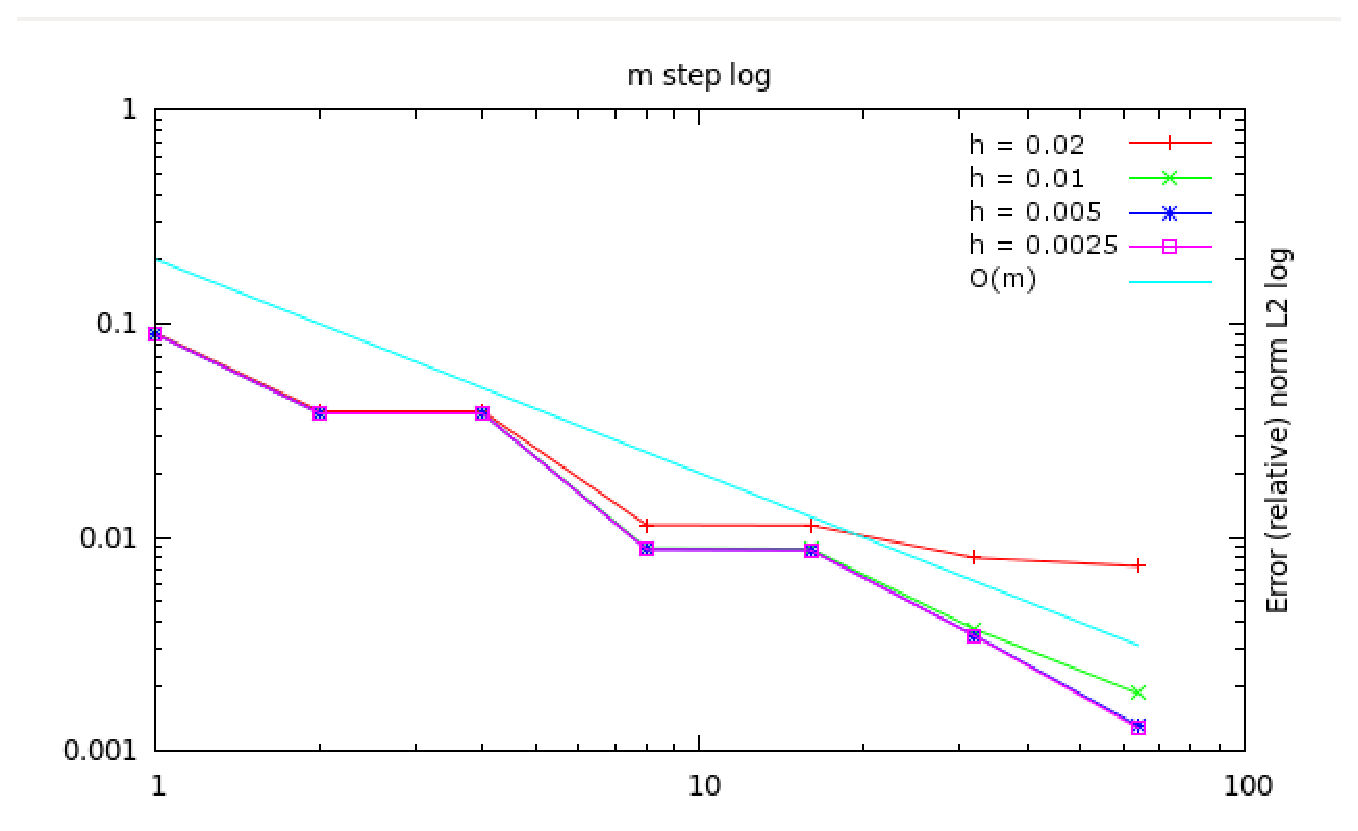
\includegraphics[scale=0.32]{Convergenze/DRDR}}{Convergenze/DRDR}}
\label{fig:drdrconv}
\end{figure}
\end{frame}

\begin{frame}
\frametitle{Convergenza RRRR}
\begin{alertblock}{}
{\footnotesize
\begin{equation}
\begin{split}
& C_1(x,y)=\frac{70}{1+x}(-\frac{2}{3L_y} y^3+ y^2) \psp{7}
C_2(x,z)=\frac{70}{1+x}(-\frac{2}{3L_z}z^3+z^2) \\
& u_{es}(x,y,z)=10^5exp( - \frac{\chi}{\mu L_y} (y - Ly/2 )^2 + C_1  - \frac{\chi}{\mu L_z}(z - L_z/2 ) ^ 2 + C_2 )(Lx-x)^2 
\end{split}
\end{equation}
}\end{alertblock}
\begin{figure}[!h]
\centering
{\linkimage{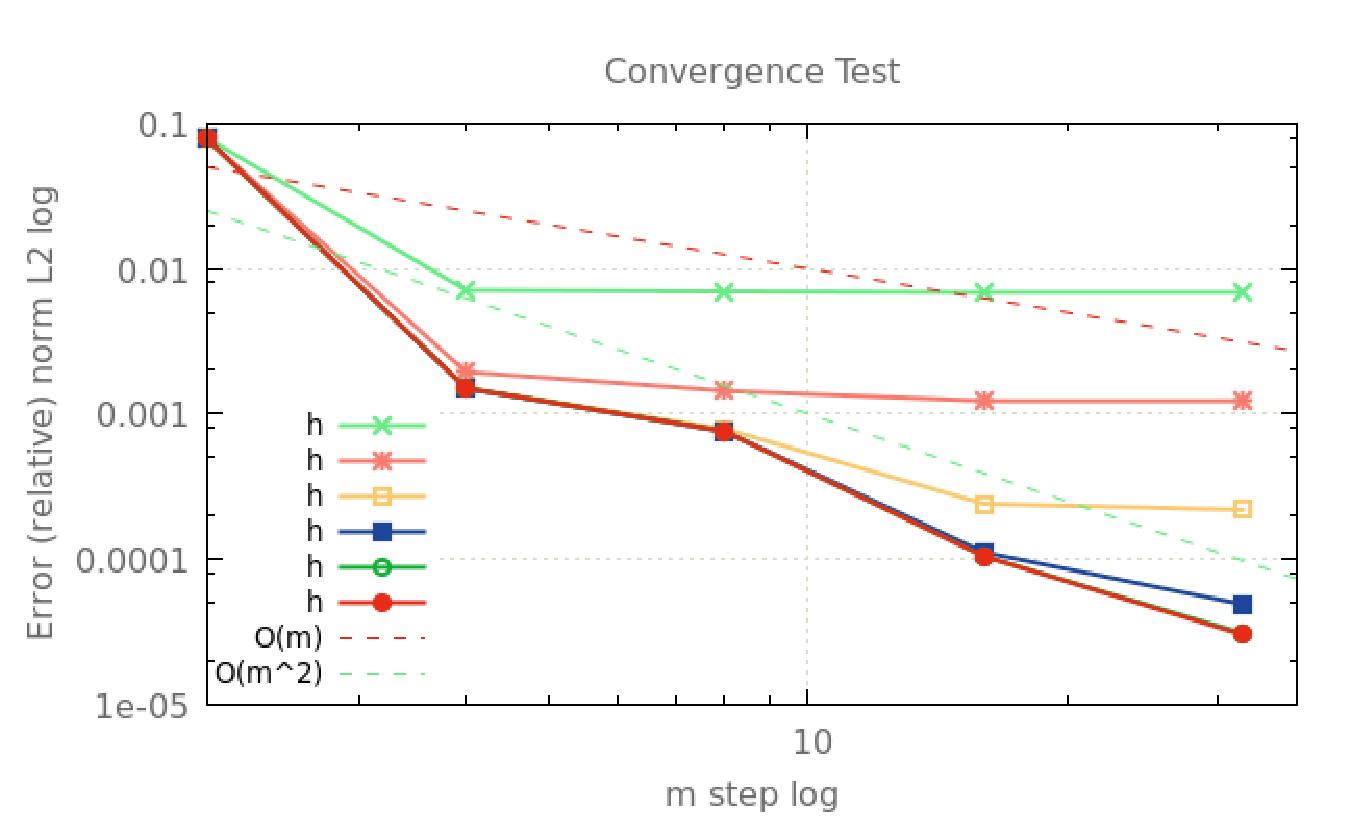
\includegraphics[scale=0.32]{Convergenze/RRRR}}{Convergenze/RRRR}}
\end{figure}

\end{frame}

\begin{frame}
\frametitle{Test camini}
\begin{columns}
\quad
\begin{column}{0.5 \paperwidth}
\begin{block}{}
\vspace{-0.5cm}
\begin{center}
\begin{equation}
\begin{cases}
-\mu\Delta u + \vect{b}\cdot \nabla u + \sigma u = f & \text{in $\Omega$}\\
u=u_{in} & \text{su $\Gamma_{in}$}\\
\frac{\partial u}{\partial \vect{n}}=0 & \text{su $\Gamma_{out}$ }\\
u=0 & \text{su $\Gamma _{vaso}$} \\
\end{cases}
\end{equation}
\end{center}
\end{block}
\begin{figure}
{\linkimage{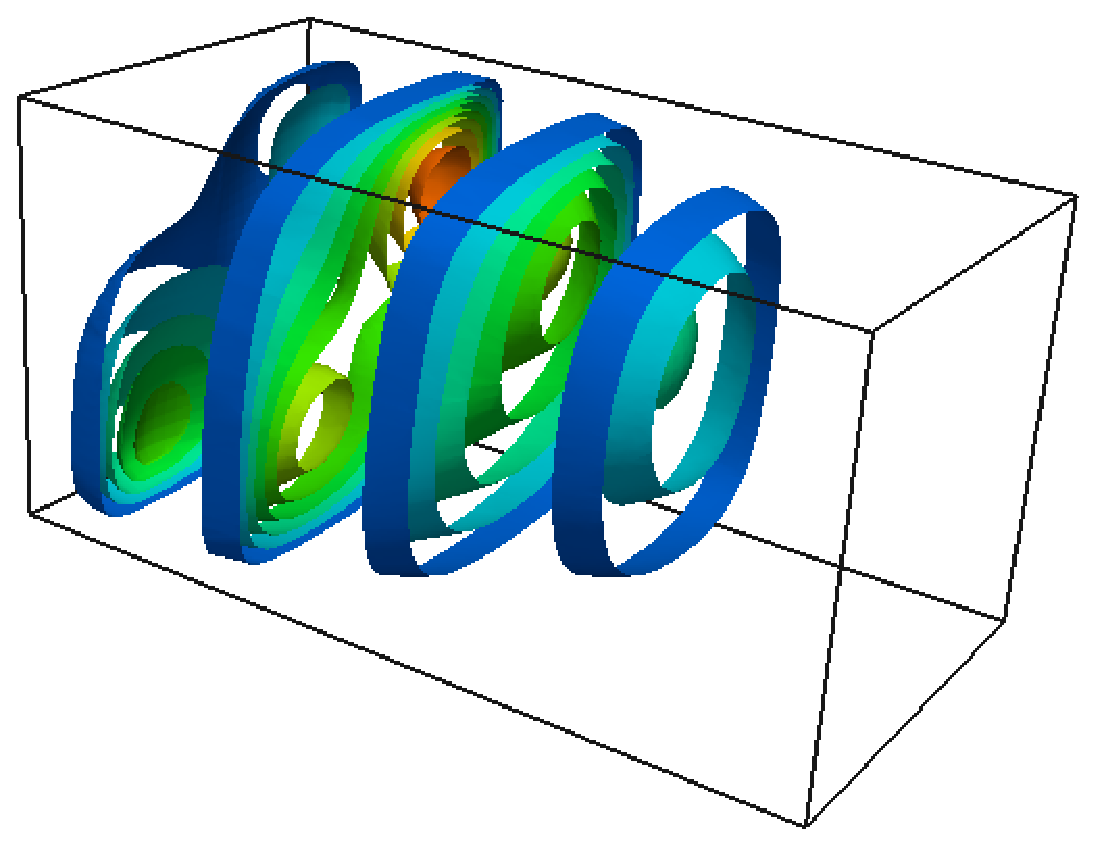
\includegraphics[scale=0.3]{Foto2D+/HiModPretty50}}{Foto2D+/HiModPretty50}}
\end{figure}
\end{column}

\begin{column}{0.5 \paperwidth}
\begin{figure}
\subfigure
{\linkimage{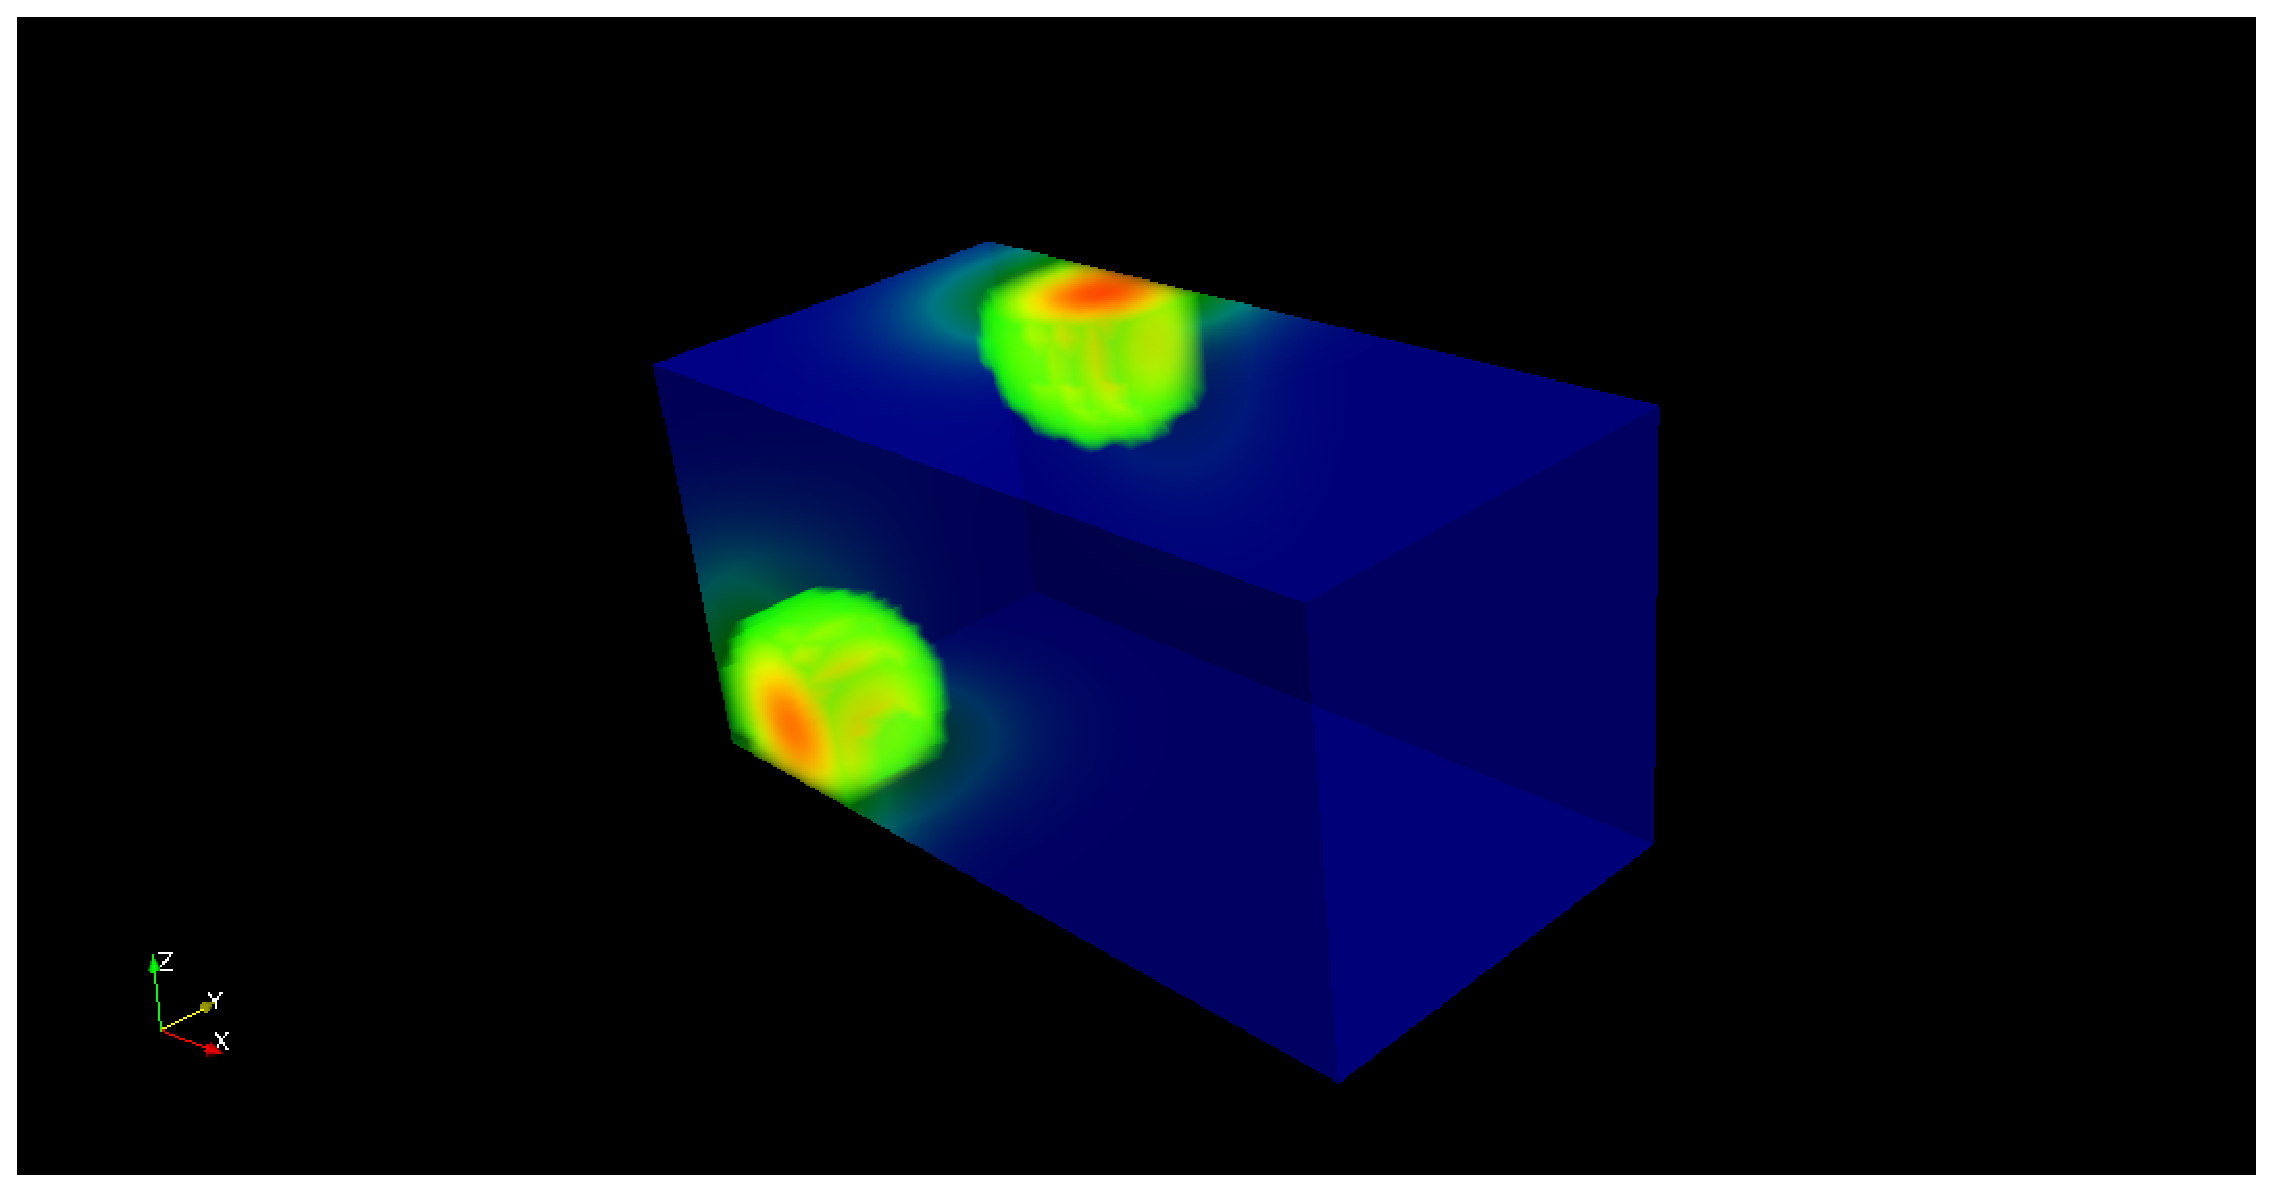
\includegraphics[scale=0.22]{DDDD_ADR/Forceterm}}{DDDD_ADR/Forceterm}}
\subfigure
{\linkimage{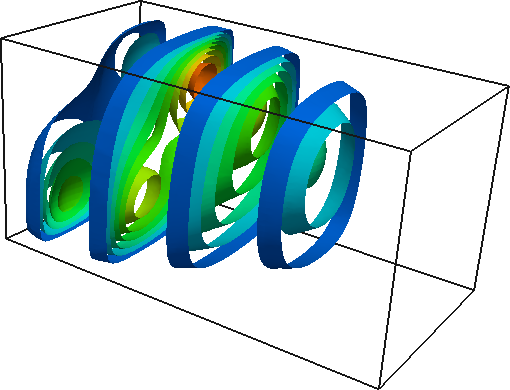
\includegraphics[scale=0.3]{Foto2D+/FEMPretty}}{Foto2D+/FEMPretty}}
\end{figure}
\end{column}

\end{columns}
\end{frame}

\begin{frame}
\frametitle{Slice XY 2D}

\begin{columns}

\begin{column}{0.5 \paperwidth}
\begin{figure}
\subfigure[m=9]
{\linkimage{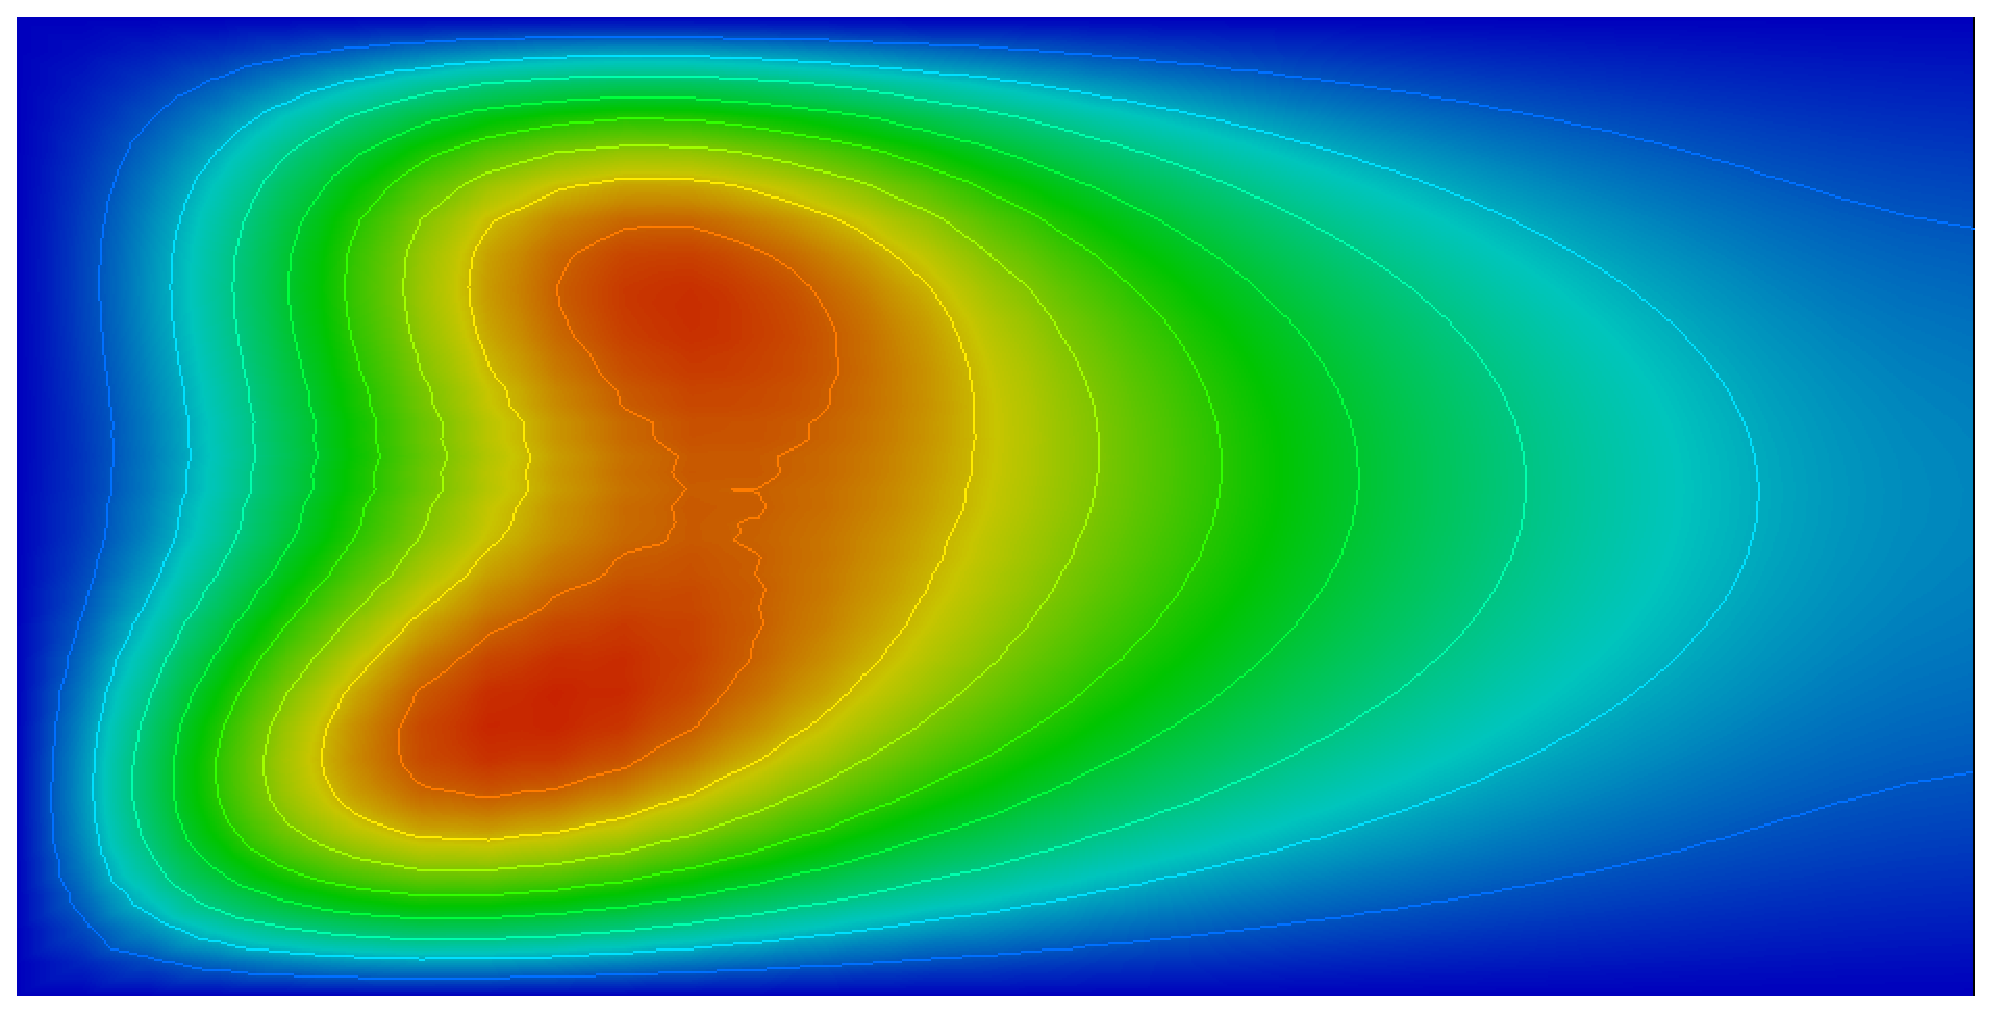
\includegraphics[height=2.8cm,width=5.5cm]{DDDD_ADR/HiMod9slice}}{DDDD_ADR/HiMod9slice}}
\subfigure[m=25]
{\linkimage{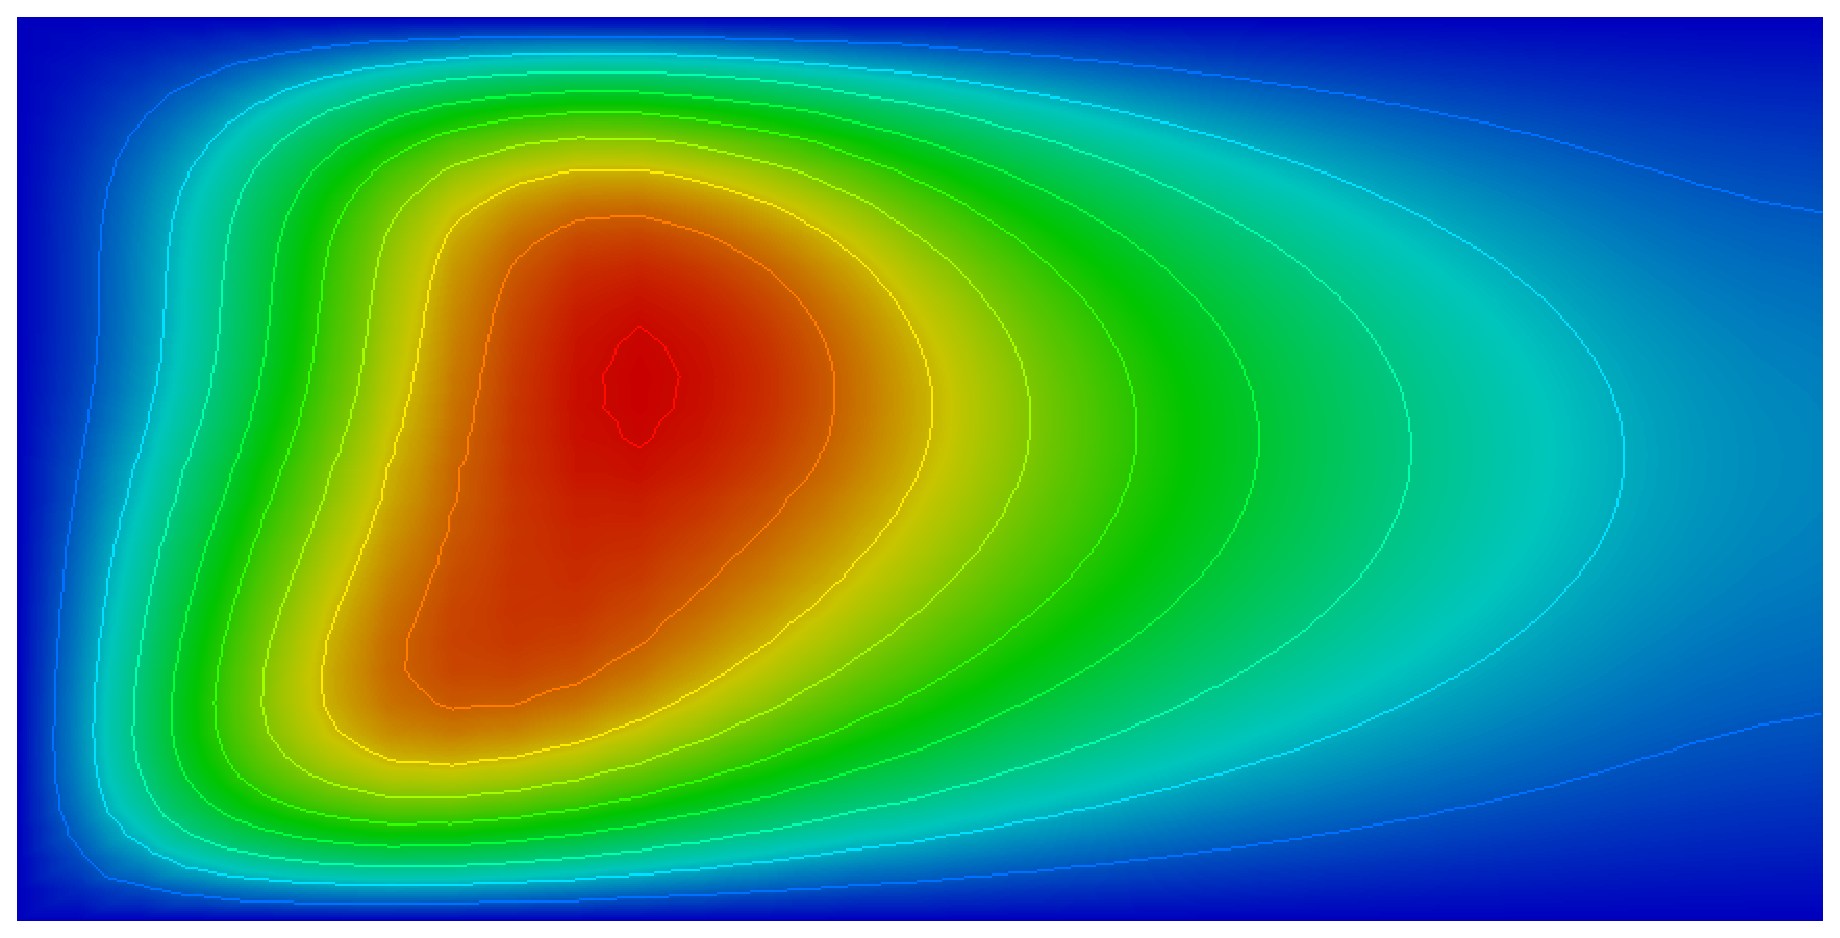
\includegraphics[height=2.8cm,width=5.5cm]{DDDD_ADR/HiMod25slice}}{DDDD_ADR/HiMod25slice}}
\end{figure}
\end{column}

\begin{column}{0.5 \paperwidth}
\begin{figure}
\subfigure[m=16]
{\linkimage{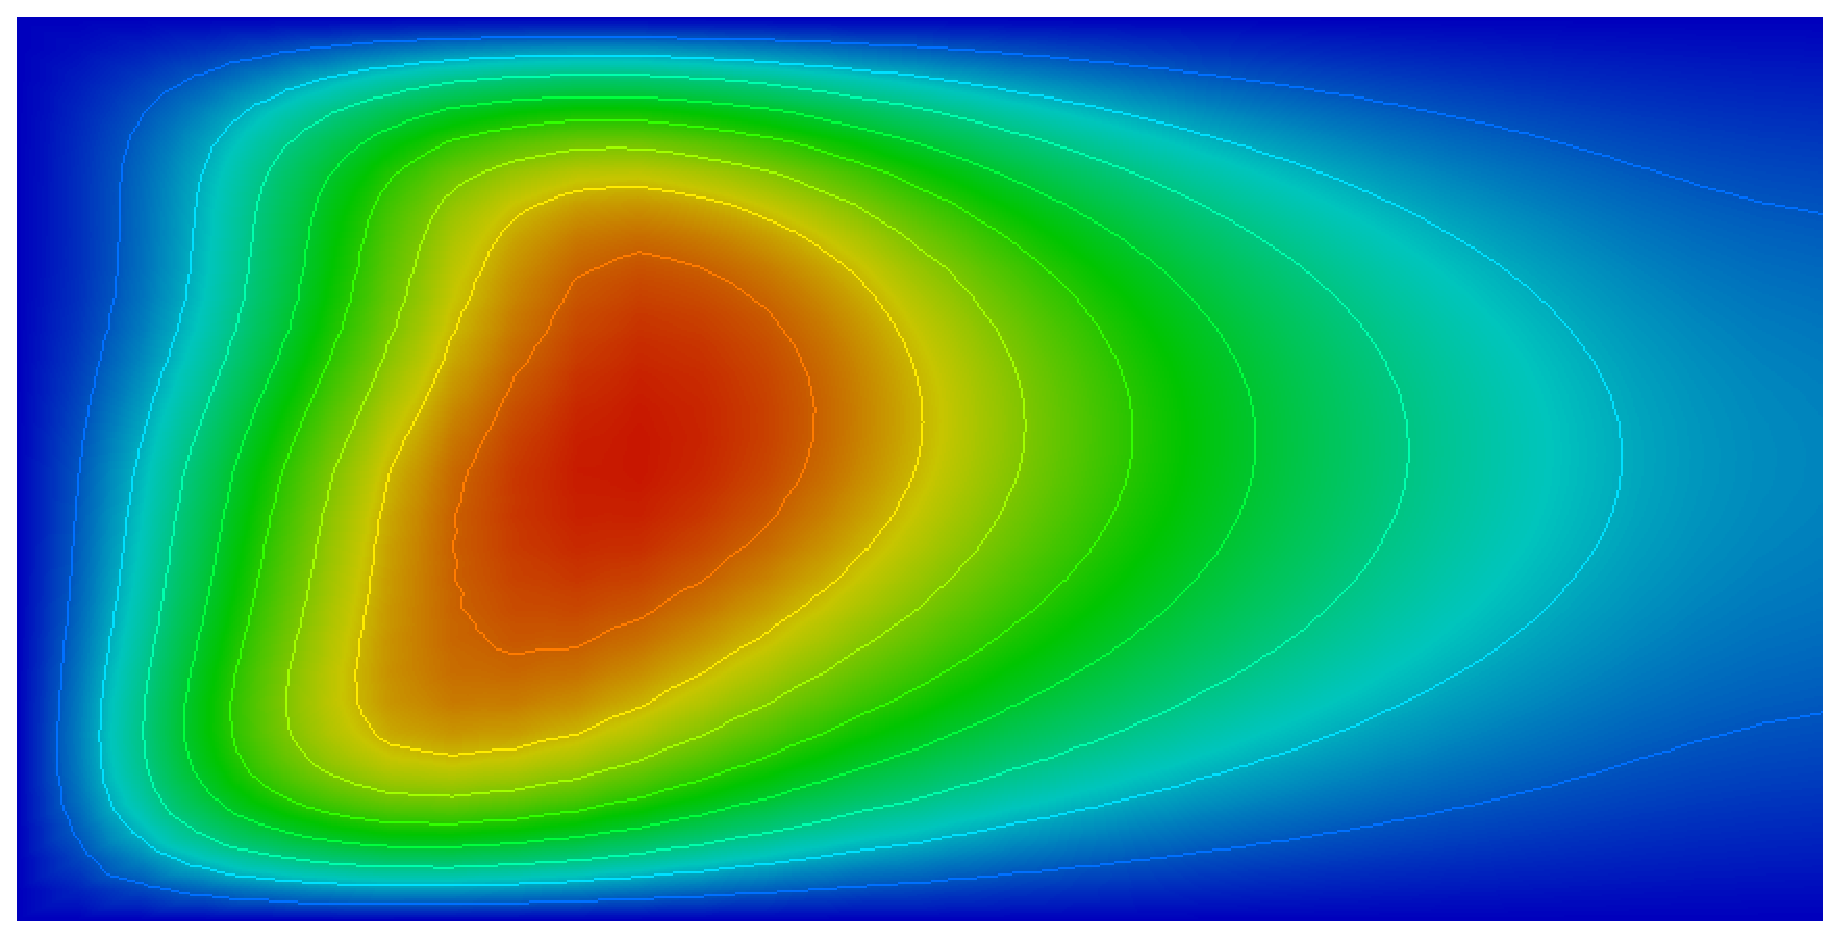
\includegraphics[height=2.8cm,width=5.5cm]{DDDD_ADR/HiMod16slice}}{DDDD_ADR/HiMod16slice}}
\subfigure[FEM]
{\linkimage{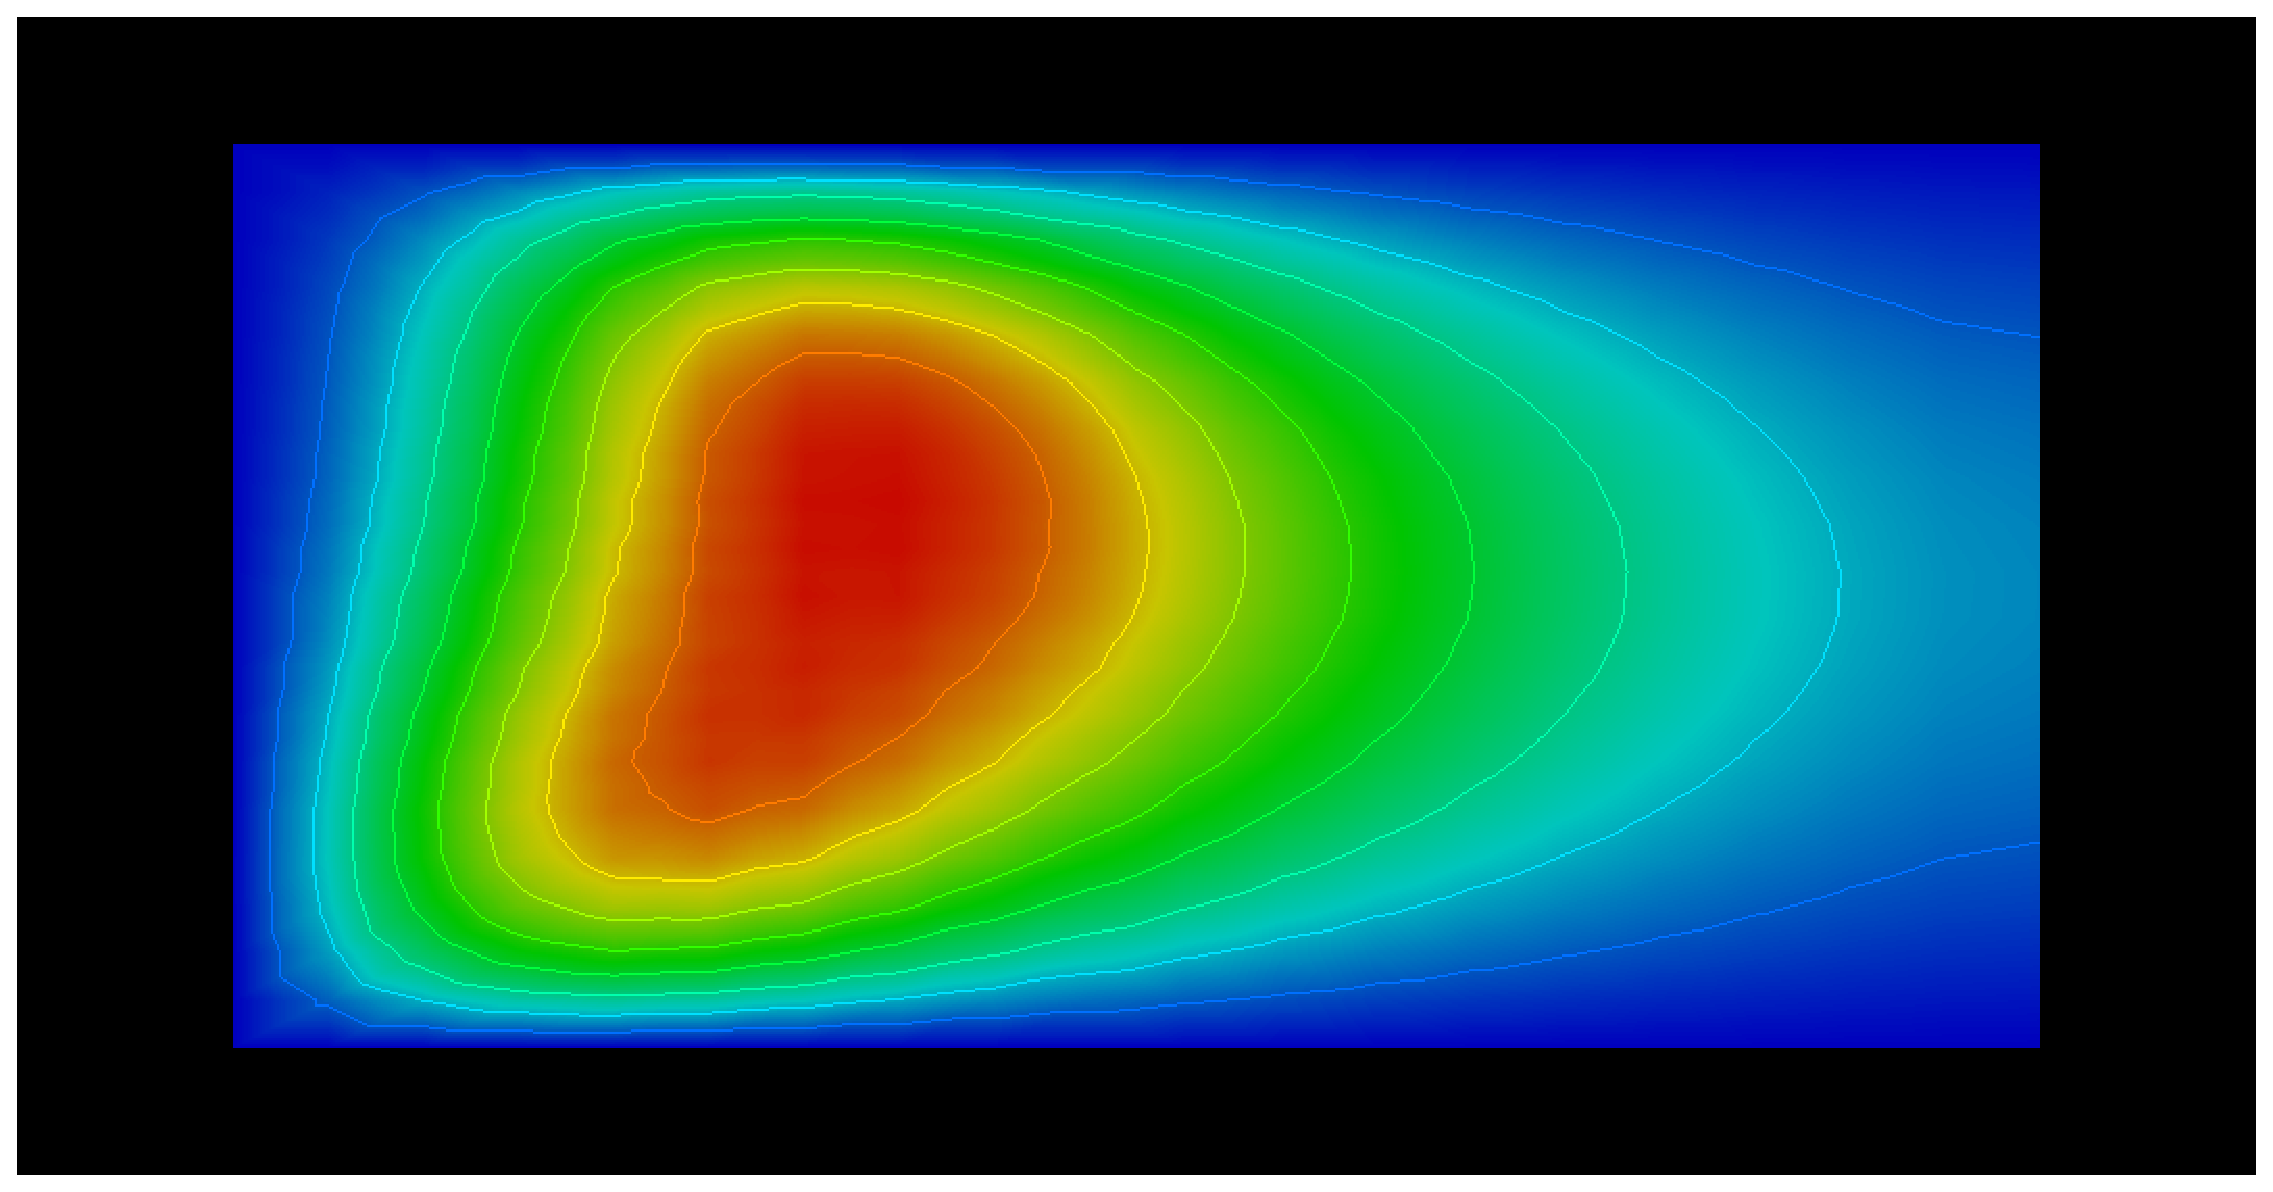
\includegraphics[height=2.8cm,width=5.5cm]{DDDD_ADR/FEMslice}}{DDDD_ADR/FEMslice}}
\end{figure}
\end{column}
\end{columns}


\end{frame}

\begin{frame}
\frametitle{Slice XY}
\begin{columns}

\begin{column}{0.5 \paperwidth}
\begin{figure}
\subfigure[m=9]
{\linkimage{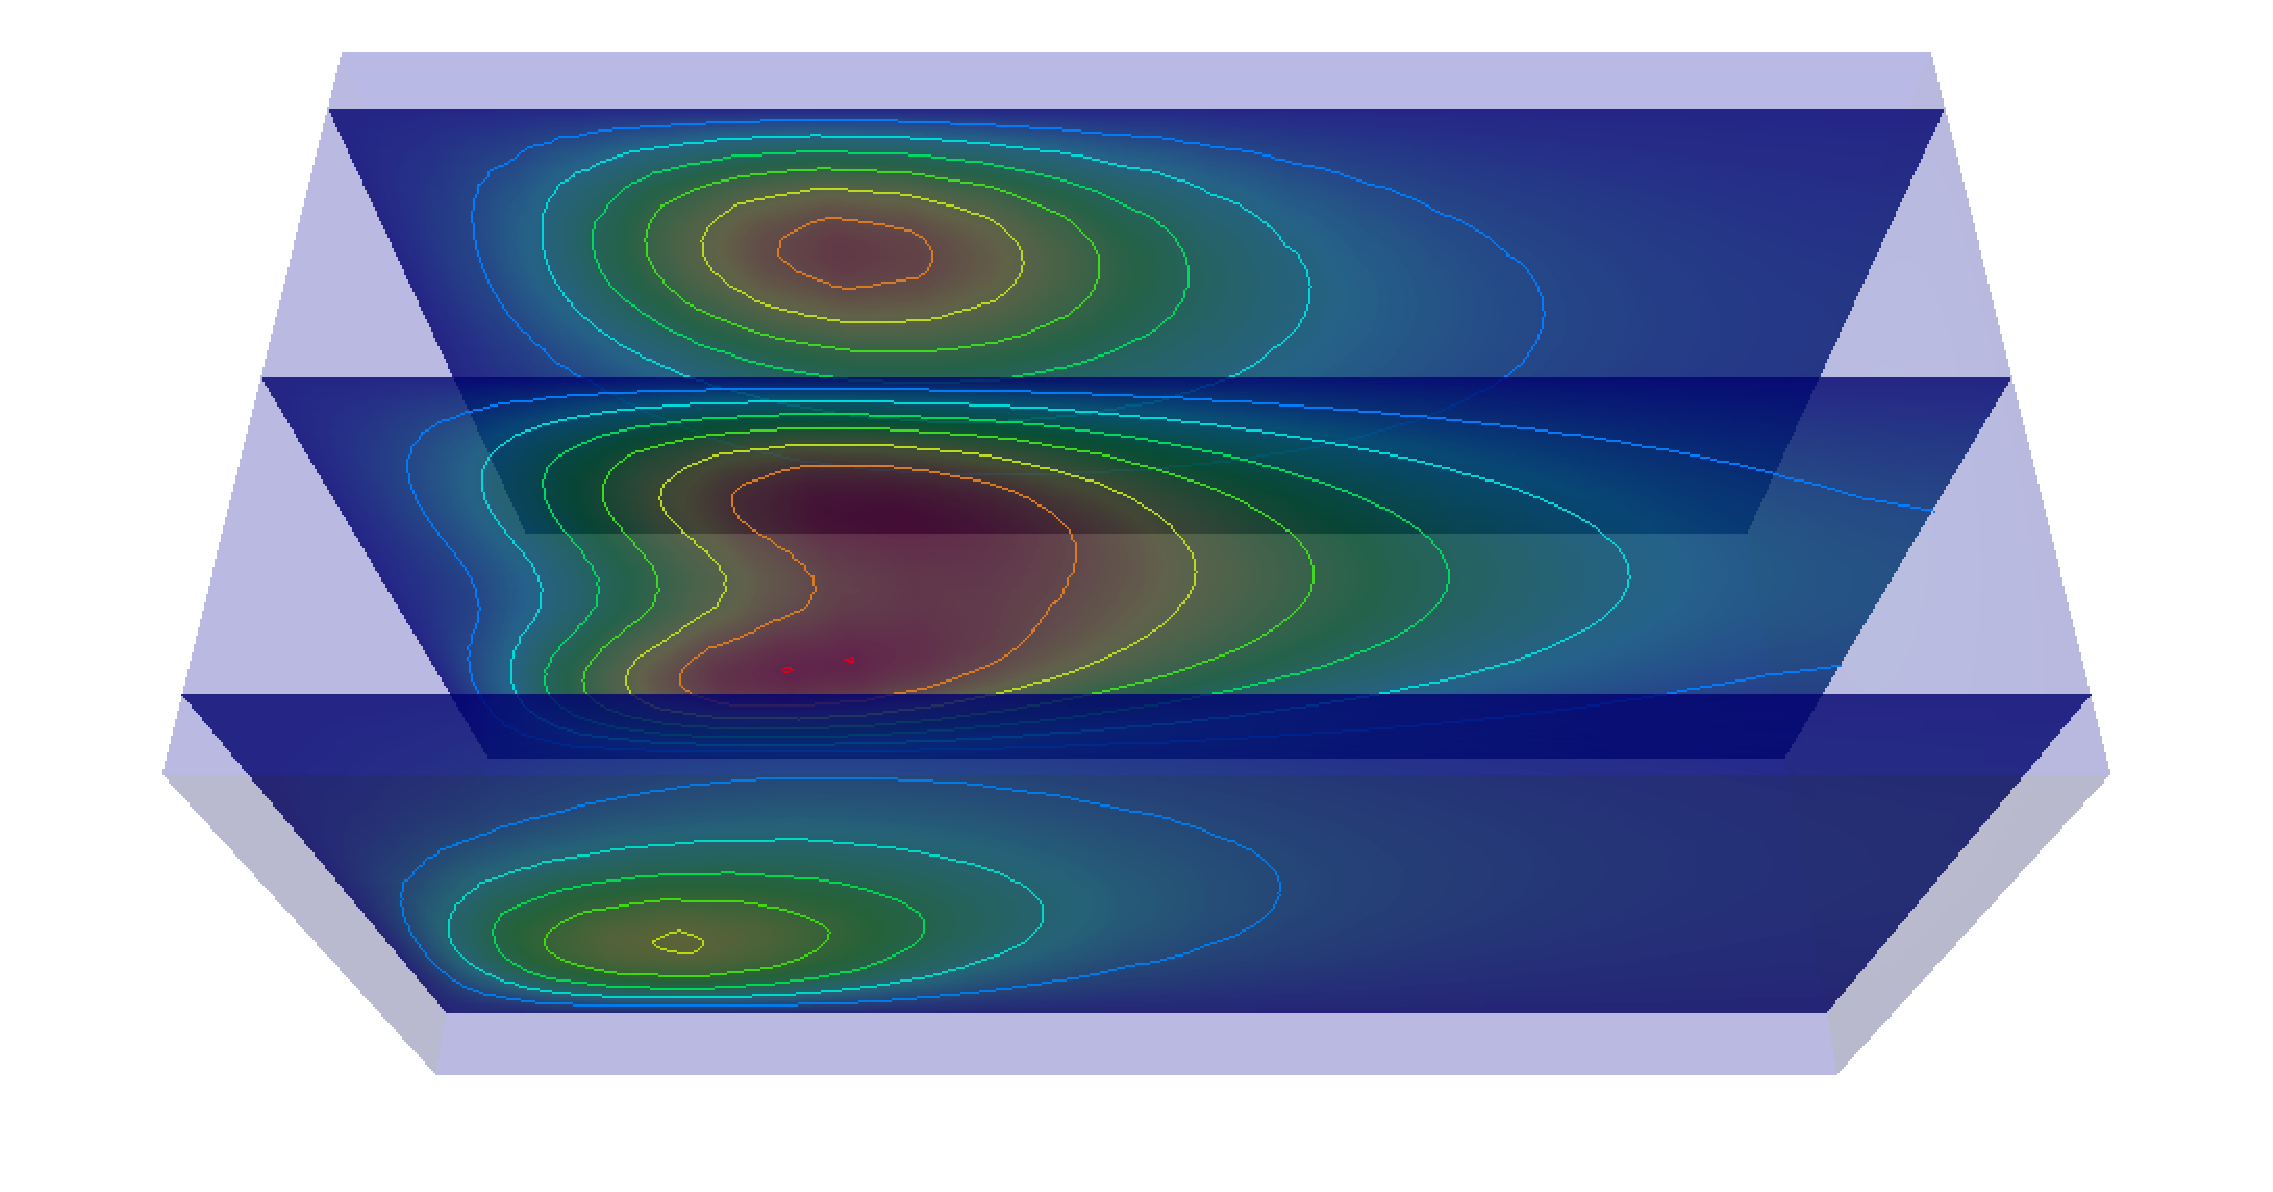
\includegraphics[scale=0.17]{Foto2D+/HiMod_m=9}}{Foto2D+/HiMod_m=9}}
\subfigure[m=25]
{\linkimage{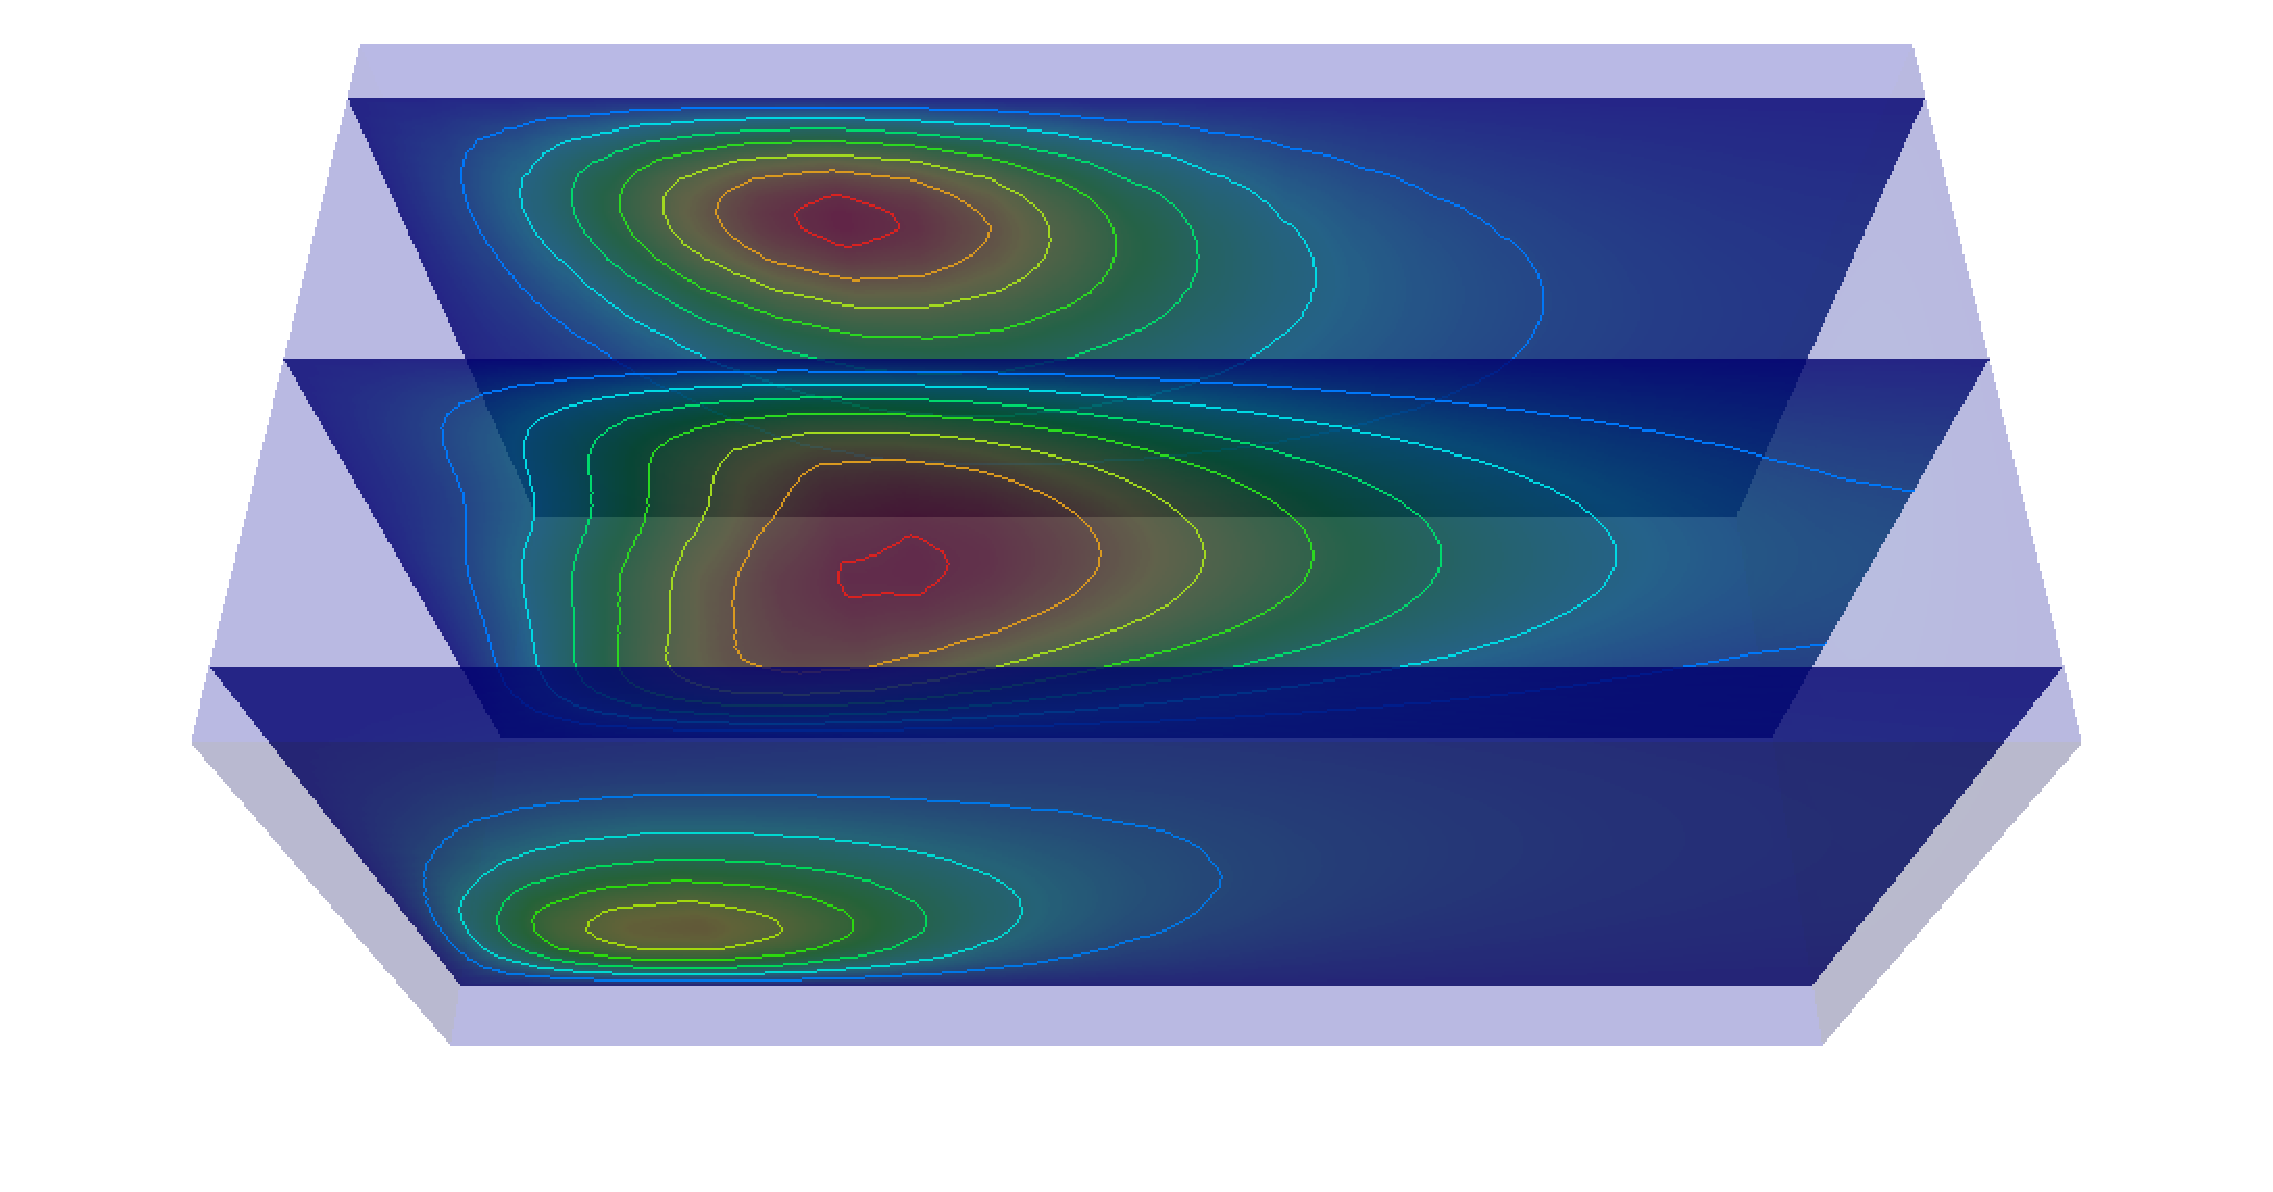
\includegraphics[scale=0.17]{Foto2D+/HiMod_m=16}}{Foto2D+/HiMod_m=16}}
\end{figure}
\end{column}

\begin{column}{0.5 \paperwidth}
\begin{figure}
\subfigure[m=16]
{\linkimage{{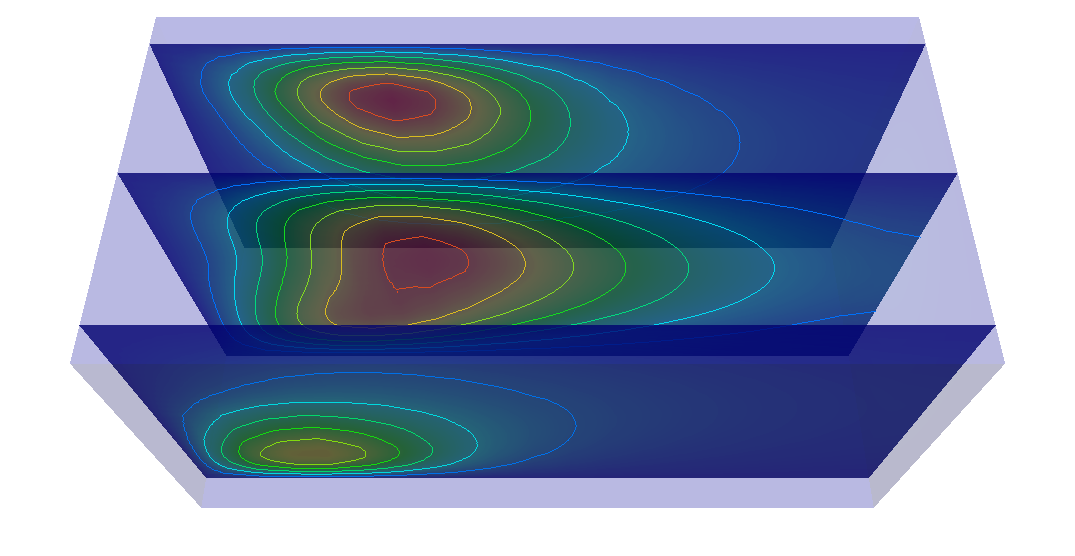
\includegraphics[scale=0.17]{Foto2D+/HiMod_m=25}}}{Foto2D+/HiMod_m=25}}
\subfigure[FEM]
{\linkimage{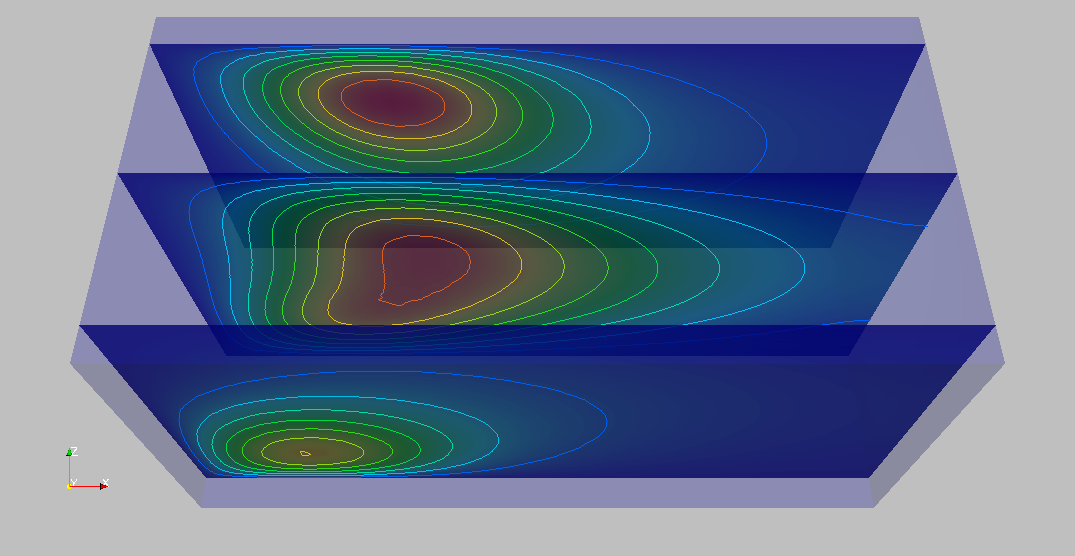
\includegraphics[scale=0.17]{Foto2D+/FEMsolution35}}{Foto2D+/FEMsolution35}}
\end{figure}
\end{column}

\end{columns}
\end{frame}

\begin{frame}
 \frametitle{Conclusioni, sviluppi futuri}
 \framesubtitle{...e work in progress}
 \begin{columns}
  \begin{column}{0.5\textwidth}
    \begin{exampleblock}<1->{Obbiettivo raggiunto!}
    HiMod consente un notevole risparmio di gradi di libert\`a.
    \end{exampleblock}
    \begin{alertblock}<2->{Work in progress}
    Generalizzazione a coefficienti non costanti e mapping.
    \end{alertblock}
  \end{column}

  \begin{column}{0.5\textwidth}
   \begin{figure}
   \centering
    {\linkimage{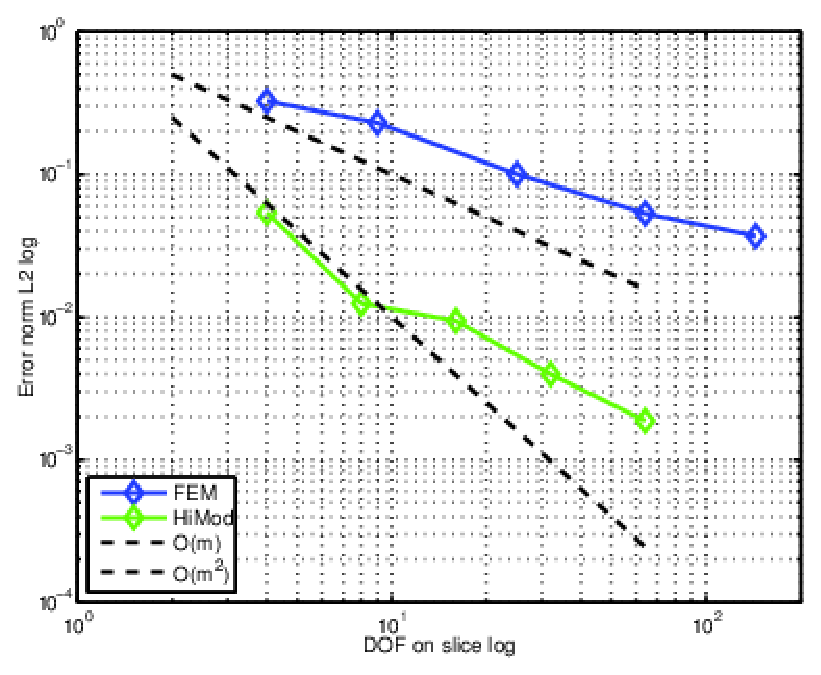
\includegraphics[scale=0.3]{Convergenze/CfrDOF}}{Convergenze/CfrDOF}}
   \end{figure}
  \end{column}
 \end{columns}
 
 \begin{block}<3->{Dove intervenire adesso?}
\begin{itemize}
\footnotesize	
    \item<4-> Sviluppo di una \textbf{struttura dati} ad hoc per la matrice di sistema
    \item<5-> \textbf{Parallelizzazione} del codice
    \item<6-> Base modale con \textbf{polinomi di Legendre}
    \item<7-> Estensione a un dominio a \textbf{sezione circolare}
    \item<8-> \textbf{Geometria generica} con la mappa
   \end{itemize}
   \end{block}
\end{frame}
\begin{frame}
 \includegraphics[scale=1]{UML/finale}
 \end{frame}
